\documentclass[11pt,a4paper]{article}

\usepackage[margin=2.05cm]{geometry}
\usepackage[T1]{fontenc}
\usepackage[utf8]{inputenc}
\usepackage{lmodern}
\usepackage{microtype}
\usepackage{amsmath,amssymb,mathtools,bm}
\usepackage{booktabs,tabularx,longtable,array,multirow}
\usepackage{graphicx}
\usepackage{caption,subcaption}
\usepackage{enumitem}
\usepackage{xcolor}
\usepackage{hyperref}
\usepackage{cleveref}
\usepackage[numbers,sort&compress]{natbib}
\usepackage{fancyhdr}
\usepackage{titlesec}
\usepackage{float}
\usepackage{siunitx}
\usepackage{url}
\usepackage[most]{tcolorbox}
\usepackage{tikz}
\usetikzlibrary{arrows.meta,positioning,fit,calc,shapes.geometric}

\definecolor{deepblue}{RGB}{28,63,105}
\definecolor{deepgreen}{RGB}{38,105,79}
\definecolor{deeporange}{RGB}{170,92,20}
\definecolor{softblue}{RGB}{232,241,250}
\definecolor{softgreen}{RGB}{235,247,240}
\definecolor{softorange}{RGB}{253,243,226}
\definecolor{softred}{RGB}{252,235,235}
\definecolor{softgray}{RGB}{245,246,248}
\definecolor{deepred}{RGB}{145,52,52}

\hypersetup{
  colorlinks=true,
  linkcolor=deepblue,
  citecolor=deepgreen,
  urlcolor=deeporange,
  pdftitle={Geometry-MMALS G1: Status and Perspective after the Context-Bottleneck Study},
  pdfauthor={Guillaume Harbonnier}
}

\pagestyle{fancy}
\fancyhf{}
\lhead{Geometry-MMALS G1}
\rhead{Reviewer status and perspective v1.1}
\cfoot{\thepage}
\setlength{\headheight}{14pt}

\titleformat{\section}{\Large\bfseries\color{deepblue}}{\thesection}{0.8em}{}
\titleformat{\subsection}{\large\bfseries\color{deepgreen}}{\thesubsection}{0.8em}{}
\titleformat{\subsubsection}{\normalsize\bfseries\color{deeporange}}{\thesubsubsection}{0.8em}{}

\setlist[itemize]{leftmargin=1.5em,itemsep=2pt,topsep=3pt}
\setlist[enumerate]{leftmargin=1.7em,itemsep=3pt,topsep=3pt}
\renewcommand{\arraystretch}{1.15}
\newcolumntype{Y}{>{\raggedright\arraybackslash}X}
\newcolumntype{C}{>{\centering\arraybackslash}X}
\newcommand{\MMALS}{\textsc{MMALS}}
\newcommand{\R}{\mathbb{R}}
\newcommand{\E}{\mathbb{E}}
\newcommand{\loss}{\mathcal{L}}
\newcommand{\norm}[1]{\left\lVert #1 \right\rVert}

\newtcolorbox{summarybox}{
  colback=softblue,colframe=deepblue!45,boxrule=0.6pt,arc=2pt,
  left=8pt,right=8pt,top=7pt,bottom=7pt
}
\newtcolorbox{positivebox}{
  colback=softgreen,colframe=deepgreen!45,boxrule=0.6pt,arc=2pt,
  left=8pt,right=8pt,top=7pt,bottom=7pt
}
\newtcolorbox{warningbox}{
  colback=softorange,colframe=deeporange!50,boxrule=0.6pt,arc=2pt,
  left=8pt,right=8pt,top=7pt,bottom=7pt
}
\newtcolorbox{criticalbox}{
  colback=softred,colframe=deepred!50,boxrule=0.6pt,arc=2pt,
  left=8pt,right=8pt,top=7pt,bottom=7pt
}

\begin{document}

\begin{titlepage}
\centering
\vspace*{0.9cm}
{\Huge\bfseries\color{deepblue} Geometry-MMALS G1\par}
\vspace{0.25cm}
{\LARGE Status, Evidence, Limitations, and Research Perspective\par}
\vspace{0.3cm}
{\Large After the v1.0.7 Context-Bottleneck Study\par}
\vspace{0.45cm}
{\large A reviewer-oriented arXiv-style technical report, version 1.1\par}
\vspace{1.0cm}
{\Large Guillaume Harbonnier\par}
\vspace{0.2cm}
{\normalsize Independent MMALS research program\par}
\vspace{0.15cm}
{\normalsize \href{https://github.com/gharbonnier78/geometry-mmalls-g1}{github.com/gharbonnier78/geometry-mmalls-g1}\par}
\vspace{0.7cm}
{\normalsize Evidence snapshot: Geometry-MMALS G1 v1.0.7, seed 0, development protocol\par}
{\normalsize June 2026\par}
\vfill
\begin{minipage}{0.92\textwidth}
\small
\textbf{Epistemic status.} This document is a reviewer-facing status and perspective synthesis, not a completed empirical qualification paper. The current evidence comes from a single controlled RotatedMNIST development seed. C0 protocol integrity is supported. The context-bottleneck study provides strong single-seed evidence that direct sensory access caused the earlier context-mediation failure, and that inferred context can drive useful and causally specific routing when forced. However, the geometry objective does not significantly improve context-space rank order or prediction, local route order is not globally aligned, curriculum sensitivity remains large, host specialization is not established, and continual memory transport is untested. No claim of quantum computation, quantum advantage, backward transfer, universal intelligence, or domain-general geometry is made.
\end{minipage}
\vfill
\end{titlepage}

\begin{abstract}
Geometry-MMALS G1 asks whether a continual-learning system composed of inferred contexts, routing distributions, functional hosts, and dual memory can acquire an internal geometry that is observable, predictive, causally controllable, and operationally useful. The program explicitly distinguishes internal functional geometry from the external geometry of audit metrics. It also imposes an evidence ladder from pipeline integrity to descriptive order, interpolation, specialization, causal control, continual transport, and operational utility.

This report consolidates the research trajectory from v1.0.0 through the executed v1.0.7 context-bottleneck experiment. The latest study resolves a major ambiguity left by v1.0.6. In the standard router, zeroing or shuffling inferred context changes accuracy by less than 0.3 percentage point, whereas removing direct sensory input from the router reduces accuracy by 4.3--7.5 points. When the router is prohibited from seeing the sensory representation, context zeroing reduces accuracy by approximately 3 points and changes the route substantially, while sensory-router interventions have exactly zero effect by construction. The context-only bottleneck remains operationally competitive: it reaches 0.658 mean interpolation accuracy and 0.600 final trained-angle accuracy, close to the standard route at 0.668 and 0.595.

The central preregistered context-geometry criterion nevertheless does not pass. Adding geometry regularization inside the context bottleneck changes trained context-order correlation by only $\Delta\rho=0.0025$ with a 95\% source-bootstrap interval $[-0.0107,0.0174]$. It does increase route order by $0.0217$ with interval $[0.0014,0.0427]$, and held-out route order by $0.0457$ with interval $[0.0092,0.0780]$. The same regularization does not improve prediction or forgetting. Moreover, local same-source route order improves while route-centroid alignment collapses from $0.489$ to $0.064$, indicating locally ordered but globally misaligned fibers. The context bottleneck yields the first strong single-seed causal-specificity result, with CSR values near 4--5, correct orientation, monotonicity, and limited identity loss, but this effect is produced mainly by architectural mediation rather than the geometry loss itself.

The reviewer-facing conclusion is therefore a mixed but scientifically informative one: the context representation is sufficient for useful, causally specific routing, and the prior mediation failure was substantially architectural. The remaining problem is an objective mismatch: the current route loss organizes local route trajectories without reliably organizing context coordinates, aligning fibers globally, or improving function. A credible empirical paper now requires direct context geometry, cross-source orientation alignment, held-out causal estimation, multiple seeds, secondary transformations, and explicit operational advantage.
\end{abstract}

\begin{summarybox}
\textbf{Reviewer recommendation in one sentence.} The work is credible as a protocol, status, or perspective paper with an unusually disciplined negative-results record; a strong empirical G1 paper still requires multi-seed evidence that context geometry is globally aligned, causally specific on held-out data, curriculum-robust, and operationally useful.
\end{summarybox}

\tableofcontents
\newpage

\section{Purpose and scope}

This document is intended for reviewers deciding whether Geometry-MMALS G1 is a coherent scientific program, whether its current evidence supports publication, and which claims remain premature. It addresses four questions:

\begin{enumerate}
\item Is the research question distinct from standard mixture-of-experts and continual-learning evaluation?
\item Which conclusions are now supported by controlled evidence, and which remain hypotheses?
\item Do the negative results narrow the hypothesis productively, or merely reveal an incoherent architecture?
\item What exact experiments separate a publishable protocol/perspective paper from a publishable empirical paper?
\end{enumerate}

The report treats implementation failures, statistical confounds, and negative controls as part of the evidence. The goal is not to maximize apparent success, but to preserve a traceable chain from hypothesis to falsification.

\section{Research question and conceptual contribution}

\subsection{From audit geometry to functional geometry}

Earlier MMALS work used vectors of observable indicators---accuracy, retention, cost, drift, host contribution, route confidence, and auditability---to compare candidate traces and select policies under changing goals. That is a useful \emph{external geometry of control}. It does not demonstrate that the learning system has organized its own representations and functions geometrically.

Geometry-MMALS G1 studies the internal chain

\begin{equation}
 x \longrightarrow z_0 \longrightarrow c \longrightarrow r
 \longrightarrow \{g_h(z_0)\}_{h=1}^{H}
 \longrightarrow z_M \longrightarrow \hat y,
\end{equation}

where $z_0$ is a frozen sensory representation, $c$ is inferred context, $r$ is a route on the host simplex, $g_h$ is host $h$'s transformation, and $z_M$ is the synthesized representation.

The central question is:

\begin{quote}
Does MMALS learn a stable relation among context, route, host function, and memory that preserves known transformation order, predicts unseen contexts, supports causal control, and improves a declared objective under continual change?
\end{quote}

This differs from standard MoE evaluation, which usually emphasizes task accuracy, sparsity, load balancing, or scale efficiency \citep{shazeer2017moe,fedus2022switch}. It also differs from purely descriptive representation analysis: a low-dimensional projection is not accepted as evidence unless it survives predictive, causal, and operational tests.

\subsection{Why the problem is geometric rather than metaphorical}

Weight-space distance is not a reliable functional metric because neural networks admit permutation, scaling, and other symmetries that can alter parameters while preserving behavior \citep{dinh2017sharp}. G1 therefore prioritizes:

\begin{itemize}
\item same-source distances under controlled transformations;
\item information geometry on routing distributions;
\item functional host distances and ablations;
\item alignment and transport across continual-learning stages;
\item interventions that test whether a latent direction changes routing in the declared way.
\end{itemize}

The program is related to information geometry \citep{amari1998natural}, latent Riemannian geometry \citep{arvanitidis2018latent,shao2018riemannian}, representation similarity \citep{kornblith2019cka}, and geometric deep learning \citep{bronstein2021geometric}. Its proposed object is more specific: a \emph{context-route-function geometry under continual change}.

\subsection{Philosophical status}

The project adopts a restrained structural perspective. It does not claim that geometry is the substance of intelligence. It claims that if a learning system genuinely uses relations among contexts, routes, and functions, then those relations should have stable, testable structure. This is closer to structural realism \citep{worrall1989structural} and interventionist causation \citep{woodward2003making} than to metaphorical naturalism. The geometry is accepted only when it constrains predictions and interventions.

\subsection{Potential novelty}

The most defensible novelty is the conjunction of six design commitments:

\begin{enumerate}
\item a frozen sensory boundary, preventing perceptual geometry from being attributed automatically to MMALS;
\item same-source cross-context measurement, separating transformation geometry from class identity;
\item an evidence ladder that separates description, prediction, causality, specialization, transport, and utility;
\item ecological host specialization defined by function and ablation rather than route frequency;
\item explicit static-route and mediation controls;
\item continual geometric transport treated as a future claim rather than a synonym for retention.
\end{enumerate}

\section{Mathematical model}

\subsection{Route geometry}

For $H$ hosts, a route is a probability vector

\begin{equation}
 r(x) \in \Delta^{H-1}, \qquad r_h\ge 0, \qquad \sum_h r_h=1.
\end{equation}

Evaluation uses the Fisher--Rao distance on the simplex,

\begin{equation}
 d_{\mathrm{FR}}(r_i,r_j)
 =2\arccos\left(\sum_{h=1}^{H}\sqrt{r_{ih}r_{jh}}\right).
\end{equation}

Training uses a stable monotonic chordal distance in square-root coordinates. For source $s$ observed at factors $u_a$ and $u_b$, the paired objective encourages route distance to reflect factor distance:

\begin{equation}
 \loss_{\mathrm{route}}
 = \E_s\sum_{a<b}
 \left(d_{\sqrt\Delta}(r_{s,a},r_{s,b})-\tau(u_a,u_b)\right)^2
 + \lambda_{\mathrm{far}}\loss_{\mathrm{margin}}.
\end{equation}

The current G1-A protocol is supervised by the known rotation angle during training. The angle is not supplied to the deployed router. The study is therefore a controlled grounding experiment, not a claim of unsupervised manifold discovery.

\subsection{Context mediation}

The standard router receives both sensory and inferred context information:

\begin{equation}
 r_{\mathrm{std}}(x)=\operatorname{softmax}R([z_0(x),c(x)]).
\end{equation}

The v1.0.7 context bottleneck removes the direct sensory path:

\begin{equation}
 r_{\mathrm{ctx}}(x)=\operatorname{softmax}R_c(c(x)),
 \qquad c(x)=C(z_0(x)).
\end{equation}

A sensory-only capacity control is

\begin{equation}
 r_{z_0}(x)=\operatorname{softmax}R_z(z_0(x)).
\end{equation}

The bottleneck experiment separates two explanations of the earlier failure:

\begin{itemize}
\item \textbf{architectural shortcut}: context is useful, but the joint router prefers direct $z_0$;
\item \textbf{representational failure}: context does not contain useful structure even when forced.
\end{itemize}

\subsection{Synthesis and host function}

The synthesized representation is

\begin{equation}
 z_M(x)=\sum_{h=1}^{H} r_h(x)\,g_h(z_0(x)).
\end{equation}

A host is not specialized merely because it receives route mass. Its functional contribution is estimated by route-renormalized ablation:

\begin{equation}
 \Delta_h(x)=\log p(y\mid x)-\log p_{-h}(y\mid x).
\end{equation}

A credible specialization claim requires localized positive contribution, reproducibility after cross-seed host matching, and stability through learning stages.

\subsection{Local fibers and global alignment}

G1 measures geometry at two levels. For each source image, the sequence of transformed observations defines a local trajectory or fiber. Source-level order asks whether

\begin{equation}
 |u_a-u_b| < |u_c-u_d|
 \quad\Rightarrow\quad
 d(r_{s,a},r_{s,b}) < d(r_{s,c},r_{s,d})
\end{equation}

on average. Global alignment asks whether trajectories from different sources share a common orientation, approximated by factor-centroid geometry. A model can improve local order while degrading centroid order; v1.0.7 demonstrates exactly this possibility.

\subsection{Retention anchor}

The present anchor is controlled rehearsal over previously seen views already present in a paired batch:

\begin{equation}
 \loss = \loss_{\mathrm{current}}
 + \lambda_{\mathrm{anchor}}\loss_{\mathrm{old\ views}}
 + \lambda_{\mathrm{route}}\loss_{\mathrm{route}}
 + \lambda_{\mathrm{div}}\loss_{\mathrm{host}}.
\end{equation}

It is not yet MMALS reconstructive memory or synthetic compiled memory. Its purpose is to test whether functional evidence stabilizes route meaning.

\subsection{Causal specificity}

A context direction $t_c$ associated with increasing angle is estimated from trained contexts. The route response is projected onto a route-angle direction $t_r$. The causal specificity ratio is

\begin{equation}
 \mathrm{CSR}
 =\frac{|\E\langle \Delta\sqrt r(t_c),t_r\rangle|}
 {\E_{q\perp t_c}|\langle\Delta\sqrt r(q),t_r\rangle|}.
\end{equation}

The pilot gate requires CSR $>1.5$, correct orientation, monotonic magnitude, limited class-evidence loss, and ultimately a confidence interval with lower bound above $1.0$ on held-out estimation data.

\section{Evidence ladder and claim discipline}

\begin{figure}[H]
\centering
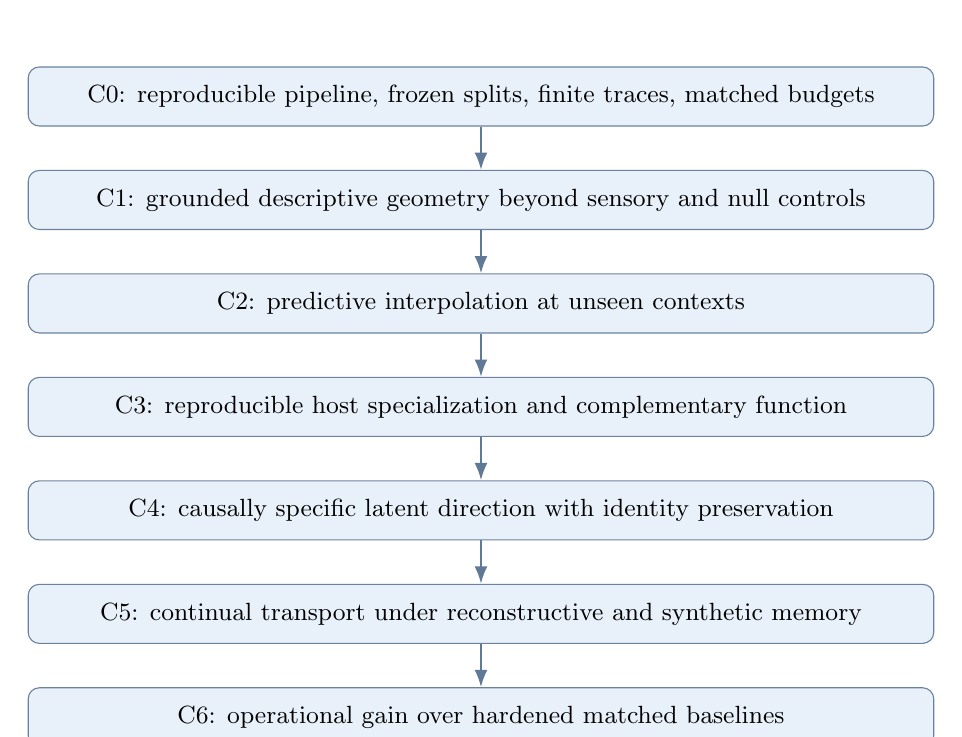
\begin{tikzpicture}[
 node distance=0.55cm,
 every node/.style={font=\small},
 box/.style={draw=deepblue!65,rounded corners,fill=softblue,minimum width=11.5cm,minimum height=0.75cm,align=center},
 arr/.style={-{Latex[length=2.2mm]},thick,deepblue!70}
]
\node[box] (c0) {C0: reproducible pipeline, frozen splits, finite traces, matched budgets};
\node[box,below=of c0] (c1) {C1: grounded descriptive geometry beyond sensory and null controls};
\node[box,below=of c1] (c2) {C2: predictive interpolation at unseen contexts};
\node[box,below=of c2] (c3) {C3: reproducible host specialization and complementary function};
\node[box,below=of c3] (c4) {C4: causally specific latent direction with identity preservation};
\node[box,below=of c4] (c5) {C5: continual transport under reconstructive and synthetic memory};
\node[box,below=of c5] (c6) {C6: operational gain over hardened matched baselines};
\draw[arr] (c0)--(c1);\draw[arr] (c1)--(c2);\draw[arr] (c2)--(c3);
\draw[arr] (c3)--(c4);\draw[arr] (c4)--(c5);\draw[arr] (c5)--(c6);
\end{tikzpicture}
\caption{Geometry-MMALS evidence ladder. Passing a lower level does not imply the next one.}
\label{fig:ladder}
\end{figure}

This ladder prevents three common overclaims: a projection is not a geometry proof; geometric order is not automatically causal; and causal control is not automatically useful continual learning.

\section{Research history: what each revision corrected}

\begin{longtable}{p{1.4cm}p{4.0cm}p{8.2cm}}
\toprule
\textbf{Version} & \textbf{Question} & \textbf{Outcome and scientific lesson}\\
\midrule
\endfirsthead
\toprule
\textbf{Version} & \textbf{Question} & \textbf{Outcome and scientific lesson}\\
\midrule
\endhead
v1.0.0 & Can functional geometry be specified? & Conceptual article, internal/external geometry distinction, evidence ladder, and controlled RotatedMNIST blueprint.\\
v1.0.1 & Can claims and gates be audited? & C0-only status, pilot thresholds, notation bridge, dual-memory contracts, and explicit supervised G1-A labeling.\\
v1.0.2 & Can the route loss train without numerical failure? & Fisher--Rao derivative instability identified; stable square-root-simplex training and finite-value guards added.\\
v1.0.3 & Does a geometry batch contain genuine cross-angle evidence? & Same-source multi-angle batches introduced. First informative run; exposed initialization and compute confounds.\\
v1.0.4 & Does geometry add value under matched initialization and compute? & Geometry improved route alignment modestly; retention anchoring improved function; context bypass and static-route questions emerged.\\
v1.0.5 & Is routing context-mediated, and does curriculum matter? & Joint router dominated by direct sensory input; static-like routing could outperform it; curriculum effects were large but terminal-task confounded.\\
v1.0.6 & Does adaptive routing beat static mixtures under same-final-task curricula? & Uniform and learned-static controls added. Strong route-order effect, weak predictive effect, sensory shortcut confirmed, and order sensitivity remained.\\
v1.0.7 & Is context failure architectural or representational? & Dedicated context and sensory bottlenecks. Context proved sufficient and causally specific when forced, but geometry did not significantly improve context order and reduced global alignment.\\
\bottomrule
\end{longtable}

The revision history is scientifically relevant because each new control was triggered by a failed assumption. Later experiments often weakened earlier interpretations rather than merely adding favorable evidence.

\section{Current experiment: v1.0.7 context bottleneck}

\subsection{Controlled factor, splits, and sensory gate}

The controlled factor is rotation. Training angles are $-60,-30,0,30,60$ degrees. Interpolation uses $-45,-15,15,45$ degrees; extrapolation uses $-75$ and $75$ degrees. The development run uses 512 training sources and 256 test sources. The frozen sensory encoder reaches $93.5\%$ test accuracy at $0$ degrees, above the $85\%$ development gate.

\subsection{Six equal-compute variants}

All methods use 15,360 forwarded images, 80 optimizer steps, the same source order, identical initialization, and the same anchor weight except the static policy's lack of instance dependence.

\begin{table}[H]
\centering
\small
\begin{tabularx}{\textwidth}{p{4.0cm}Yccc}
\toprule
\textbf{Variant} & \textbf{Router input} & \textbf{Geo} & \textbf{Anchor} & \textbf{Purpose}\\
\midrule
Standard anchor & $[z_0,c]$ & 0 & 0.10 & v1.0.6 baseline with shortcut available\\
Uniform static & none & 0 & 0.10 & fixed-mixture operational floor\\
Context bottleneck & $c$ only & 0 & 0.10 & context sufficiency\\
Context bottleneck + geometry & $c$ only & 0.10 & 0.10 & primary context-geometry contrast\\
Sensory bottleneck & $z_0$ only & 0 & 0.10 & capacity and information-path control\\
Sensory bottleneck + geometry & $z_0$ only & 0.10 & 0.10 & sensory geometry control\\
\bottomrule
\end{tabularx}
\caption{Controlled v1.0.7 variants.}
\end{table}

The primary falsification condition was preregistered: if geometry regularization inside the context bottleneck failed to increase context-space rank order with a confidence interval excluding zero, the context-geometry claim would not pass.

\section{Empirical status}

\subsection{Protocol and release integrity}

The v1.0.7 manifest records notebook and package version 1.0.7, Git commit \texttt{b06a303...}, source hashes, split hashes, initial-state hash, method specifications, parameter counts, and tracked changes. All finite-value and compute assertions passed. C0 is therefore supported for this development run, but C1--C6 remain separate claims.

\subsection{The sensory shortcut is real}

For the standard router, zeroing inferred context changes accuracy by $+0.22$ percentage point and shuffling it by $+0.13$ point. In contrast, zeroing the router's $z_0$ input reduces accuracy by $4.30$ points, and shuffling it reduces accuracy by $7.47$ points. The context-to-sensory route-shift ratio is only $0.032$.

\begin{figure}[H]
\centering

\includegraphics[width=0.88\textwidth]{../figures/mediation_accuracy_deltas_v107.pdf}
\caption{Router-only intervention effects. Host transformations still receive $z_0$; only the router input is changed.}
\label{fig:mediation}
\end{figure}

\begin{criticalbox}
\textbf{Reviewer-relevant diagnosis.} The standard architecture does not demonstrate context-mediated routing. It learns a direct sensory shortcut and can nearly ignore the inferred context variable.
\end{criticalbox}

\subsection{Forced context mediation works}

The context bottleneck changes the interpretation. With no geometry loss, context zeroing reduces accuracy from $0.6259$ to $0.5946$ and shifts the route by $0.394$. With geometry, context zeroing reduces accuracy from $0.6207$ to $0.5911$ and shifts the route by $0.349$. Sensory-router interventions have exactly zero effect because $z_0$ is structurally unavailable to the router.

The context-only router remains operationally competitive:

\begin{table}[H]
\centering
\small
\begin{tabular}{lccc}
\toprule
\textbf{Method} & \textbf{Interpolation acc.} & \textbf{Final trained acc.} & \textbf{Forgetting}\\
\midrule
Standard $[z_0,c]$ & 0.6680 & 0.5953 & 0.0992\\
Uniform static & 0.6367 & 0.5867 & 0.1234\\
Context bottleneck & 0.6582 & \textbf{0.6000} & 0.1109\\
Context bottleneck + geo & 0.6553 & 0.5930 & 0.1156\\
Sensory bottleneck & 0.6523 & 0.5836 & 0.1195\\
Sensory bottleneck + geo & 0.6650 & 0.5930 & 0.1109\\
\bottomrule
\end{tabular}
\caption{Operational results under matched compute.}
\label{tab:perf}
\end{table}

\begin{positivebox}
\textbf{Admissible current claim.} The inferred two-dimensional context contains sufficient information to drive a competitive adaptive route when direct sensory access is prohibited.
\end{positivebox}

This rejects the strong representational-failure hypothesis. The earlier mediation failure was substantially architectural.

\subsection{The preregistered context-geometry criterion fails}

The primary comparison is context bottleneck plus geometry versus context bottleneck without geometry.

\begin{figure}[H]
\centering

\includegraphics[width=0.72\textwidth]{../figures/context_bottleneck_geometry_trained.pdf}
\caption{Paired-source geometry effect on trained angles. Error bars are source-bootstrap 95\% intervals.}
\label{fig:geotrain}
\end{figure}

On trained angles:

\begin{itemize}
\item context: $\Delta\rho=+0.0025$, interval $[-0.0107,+0.0174]$;
\item route: $\Delta\rho=+0.0217$, interval $[+0.0014,+0.0427]$;
\item synthesis: $\Delta\rho=+0.0005$, interval $[-0.0035,+0.0051]$.
\end{itemize}

On held-out interpolation angles:

\begin{figure}[H]
\centering

\includegraphics[width=0.72\textwidth]{../figures/context_bottleneck_geometry_interpolation.pdf}
\caption{Paired-source geometry effect on held-out interpolation angles.}
\label{fig:geointerp}
\end{figure}

\begin{itemize}
\item context: $\Delta\rho=+0.0164$, interval $[-0.0087,+0.0403]$;
\item route: $\Delta\rho=+0.0457$, interval $[+0.0092,+0.0780]$;
\item synthesis: $\Delta\rho=-0.0010$, interval $[-0.0075,+0.0053]$.
\end{itemize}

The context-order intervals include zero. The preregistered C1-context success criterion therefore does not pass. Context stress improves slightly, but rank order does not improve convincingly.

\begin{warningbox}
\textbf{Interpretation.} Geometry regularization shapes the route produced from context. It does not show that the context coordinates themselves become a better ordered manifold.
\end{warningbox}

\subsection{Local order improves while global alignment collapses}

The context bottleneck without geometry has source-level route correlation $0.331$ and route-centroid correlation $0.489$. With geometry, source-level route correlation rises to $0.352$, while route-centroid correlation falls to $0.064$.

\begin{figure}[H]
\centering

\includegraphics[width=0.72\textwidth]{../figures/local_vs_global_route_alignment.pdf}
\caption{The geometry loss improves local same-source route order but degrades global route-centroid alignment.}
\label{fig:fibers}
\end{figure}

This suggests a bundle of locally ordered, source-dependent fibers rather than a single globally aligned transformation manifold. The route loss is therefore incomplete if the intended object is a common coordinate system.

\subsection{Geometry does not improve prediction}

Inside the context bottleneck, geometry changes mean interpolation accuracy by $-0.29$ point, final trained-angle accuracy by $-0.70$ point, and forgetting by $+0.47$ point. All individual interpolation confidence intervals include zero. The geometry objective is therefore representational, not operational, in this run.

The sensory-only path responds more strongly: geometry increases trained route order by $0.0835$ and held-out route order by $0.1404$, with positive intervals, and gives a modest $+1.27$ point mean interpolation gain. This indicates that the current loss is easier to exploit through a richer sensory representation than through the compressed context.

\begin{figure}[H]
\centering

\includegraphics[width=0.94\textwidth]{../figures/method_accuracy_v107.pdf}
\caption{Matched-compute performance across the six v1.0.7 route policies.}
\label{fig:accuracy}
\end{figure}

\begin{figure}[H]
\centering

\includegraphics[width=0.94\textwidth]{../figures/method_forgetting_v107.pdf}
\caption{Mean forgetting. Lower is better.}
\label{fig:forgetting}
\end{figure}

\subsection{Causal specificity changes qualitatively}

The context bottleneck produces the first strong single-seed causal candidate result.

\begin{figure}[H]
\centering

\includegraphics[width=0.82\textwidth]{../figures/causal_csr_v107.pdf}
\caption{Mean causal specificity ratio. The horizontal line is the pilot threshold.}
\label{fig:causal}
\end{figure}

The standard router has mean CSR $0.165$ and fails orientation. The context bottleneck without geometry reaches $5.40$; with geometry it reaches $4.00$. Both pass orientation and monotonicity with maximum class log-probability changes below $0.04$. Sensory-only routes produce no meaningful context-tangent effect.

This is strong candidate evidence that forced context mediation yields a specific route-control direction. However, three limitations prevent C4 qualification:

\begin{enumerate}
\item tangent estimation and testing occur within the same run;
\item no source-bootstrap interval is reported for CSR;
\item only one seed and one transformation are available.
\end{enumerate}

Geometry is not the cause of the causal improvement; CSR is actually higher without the geometry term. Architectural mediation is the main intervention.

\subsection{Curriculum sensitivity remains dominant}

All four curricula end at $30$ degrees, removing the earlier terminal-task confound. Performance still varies substantially.

\begin{figure}[H]
\centering

\includegraphics[width=0.78\textwidth]{../figures/curriculum_accuracy_v107.pdf}
\caption{Final trained-angle and interpolation accuracy across same-final-task curricula.}
\label{fig:curracc}
\end{figure}

\begin{figure}[H]
\centering

\includegraphics[width=0.72\textwidth]{../figures/curriculum_forgetting_v107.pdf}
\caption{Mean forgetting across same-final-task curricula.}
\label{fig:currforget}
\end{figure}

The primary order \texttt{cb\_a} yields forgetting $0.116$, final accuracy $0.593$, and interpolation $0.655$. The best order, \texttt{cb\_b}, yields $0.048$, $0.640$, and $0.718$. Center-first or near-center-first schedules outperform extreme-first schedules. The curriculum effect is much larger than the geometry-loss effect.

\subsection{Host ecology remains suggestive, not specialized}

The context bottleneck uses mainly hosts 1 and 3. Geometry shifts route mass from host 1 toward host 3, but positive ablation fractions remain close to chance for many regions. This is route rebalancing, not reproducible local specialization. C3 still requires cross-seed host matching, locality ratios, replacement controls, and role stability across curricula.

\subsection{Parameter accounting}

The manifest reports router-module parameters of 4,612 for the context bottleneck, 8,644 for the standard router, and 12,676 for the sensory bottleneck. The trainable context encoder adds approximately 8,386 parameters. The complete context mediation path is therefore approximately 12,998 parameters, close to the sensory path. Future manifests should report both module-only and end-to-end mediation-path counts to avoid a misleading capacity interpretation.

\section{Integrated interpretation}

\subsection{What v1.0.7 establishes}

The strongest coherent interpretation is:

\begin{enumerate}
\item the earlier context failure was substantially caused by an architectural sensory shortcut;
\item the inferred context contains enough information for useful adaptive routing;
\item forced context routing supports a highly specific single-seed causal direction;
\item the current geometry objective improves route order, not context rank order;
\item local route geometry can improve while global alignment deteriorates;
\item geometric order remains disconnected from prediction benefit;
\item curriculum order remains a first-order determinant of performance.
\end{enumerate}

This is best described as an \emph{architectural mediation success with a geometry-objective mismatch}.

\subsection{Why this is not a negative dead end}

The context-bottleneck result rejects the most damaging interpretation: that the context variable is intrinsically useless. It narrows the problem from ``does context exist?'' to ``how should context geometry be supervised and aligned?'' That is a much more precise research target.

The negative result also separates three notions that were previously conflated:

\begin{itemize}
\item \textbf{context sufficiency}: context can drive a useful route;
\item \textbf{route geometry}: route distances can reflect transformation order;
\item \textbf{context geometry}: context coordinates themselves form a stable, globally aligned structure.
\end{itemize}

v1.0.7 supports the first, gives candidate evidence for the second, and does not support the third.

\subsection{Local fibers as a revised conceptual model}

The evidence suggests that a single global manifold may be too strong an initial model. A more plausible structure is a fiber bundle:

\begin{itemize}
\item source identity or class defines a base point or local chart;
\item transformation produces a local trajectory within that chart;
\item routing can be locally ordered without sharing a common global orientation;
\item alignment requires an additional cross-source transport or gauge-fixing mechanism.
\end{itemize}

This interpretation is compatible with geometric deep-learning ideas about local charts and gauges \citep{bronstein2021geometric}, but it remains an inference from the current metrics, not a proved mathematical structure.

\section{What is established, promising, failed, or untested}

\begin{table}[H]
\centering
\small
\begin{tabularx}{\textwidth}{p{3.8cm}p{2.5cm}Y}
\toprule
\textbf{Claim} & \textbf{Status} & \textbf{Evidence}\\
\midrule
C0 protocol integrity & Established, development & Version, hashes, splits, matched compute, finite traces, exports, and sensory gate passed.\\
Sensory shortcut diagnosis & Established in seed 0 & Standard router ignores context interventions but depends strongly on $z_0$.\\
Context sufficiency & Strong candidate & Context-only route remains competitive and context zeroing reduces accuracy by about 3 points.\\
Context-primary routing & Established by design and intervention & Context bottleneck has no $z_0$ route path; zeroing context changes route and function.\\
Context geometry improvement & Failed / inconclusive & Context $\Delta\rho$ intervals include zero.\\
Route geometry under bottleneck & Candidate & Positive route $\Delta\rho$ on trained and held-out partitions.\\
Global route manifold & Failed & Route-centroid correlation collapses under the geometry loss.\\
Predictive gain from geometry & Not demonstrated & Accuracy and forgetting changes are neutral or slightly negative.\\
Causal specificity & Strong single-seed candidate & CSR 4--5 with correct orientation and monotonicity; no held-out or cross-seed CI.\\
Host specialization & Not qualified & Two-host ecology, no reproducible local roles.\\
Memory transport & Not implemented & Reconstructive and synthetic memory remain outside the run.\\
Operational utility & Not qualified & No robust accuracy--retention--cost advantage across seeds and curricula.\\
Curriculum robustness & Failed & Same-final-task schedules still vary strongly.\\
\bottomrule
\end{tabularx}
\caption{Current claim status after v1.0.7.}
\end{table}

\section{Reviewer risk assessment}

\subsection{Risk 1: supervised shaping may be mistaken for discovery}

G1-A uses known angle labels in the geometry loss. The report must state this prominently. The contribution is not unsupervised discovery, but a controlled test of whether a known factor can be represented and used through the MMALS architecture.

\subsection{Risk 2: the causal probe may be circular}

The tangent and route direction are estimated from the same run used for evaluation. High CSR is therefore candidate evidence, not final causal proof. Held-out source blocks and separate tangent-estimation splits are required.

\subsection{Risk 3: local geometry may be source-specific}

The source-level gains and centroid collapse show that local order is not equivalent to a common manifold. A reviewer may reasonably ask whether the model learned many unrelated source-specific trajectories. Cross-source orientation alignment is now mandatory.

\subsection{Risk 4: context dimension may be too restrictive}

The two-dimensional context is interpretable but may compress identity and transformation too aggressively. Context dimensions $2,4,8$ should be compared under equal parameter budgets and direct context supervision.

\subsection{Risk 5: operational benefit remains absent}

Geometry changes route order but not prediction. Unless geometry reduces compute, improves calibration, improves retention, or enables control under drift, it may remain epiphenomenal.

\subsection{Risk 6: curriculum effects can dominate architecture}

Even same-final-task schedules differ substantially. Multi-seed method comparisons must include curriculum as a factor, not a fixed nuisance variable.

\subsection{Risk 7: one synthetic transformation is insufficient}

RotatedMNIST is appropriate for falsification because the factor is known, but insufficient for generality. A second controlled factor should differ structurally, such as scale, corruption severity, illumination, or continuous domain shift.

\section{Publication positioning}

\subsection{What can be published now}

A protocol, perspective, or status paper can defensibly claim:

\begin{itemize}
\item a formal distinction between audit geometry and internal context-route-function geometry;
\item a falsifiable evidence ladder with explicit non-claims;
\item same-source paired measurement, matched compute, source-bootstrap inference, static controls, and mediation controls;
\item a documented sequence of negative results that progressively narrows the hypothesis;
\item single-seed evidence that context mediation failure was architectural and that forced context routing is operationally viable and causally specific;
\item single-seed candidate evidence that route geometry can be shaped independently of context geometry and prediction.
\end{itemize}

This would be strongest as a methodological status paper, not a state-of-the-art continual-learning result.

\subsection{What is required for an empirical G1 paper}

A credible empirical submission requires at minimum:

\begin{enumerate}
\item five pilot seeds and ten final seeds, reporting failed runs;
\item direct context-geometry regularization rather than route-only regularization;
\item cross-source orientation or centroid alignment with preregistered thresholds;
\item held-out tangent estimation and source-bootstrap CSR intervals;
\item factorial curriculum analysis with method-by-order interaction;
\item context dimensions $2,4,8$ under matched end-to-end parameter budgets;
\item a validation-optimized static route and low-capacity adaptive controls;
\item a second controlled transformation or dataset;
\item an operational benefit such as improved accuracy-retention-cost trade-off, calibration, or drift recovery;
\item no C5 claim until reconstructive and synthetic memory transport are implemented.
\end{enumerate}

\subsection{What should remain separate}

The TPUT architecture paper and Geometry G1 empirical paper should remain distinct. TPUT specifies the operational loop and future energy-guided control. G1 qualifies whether the internal geometry required by that loop exists. Phase-aware or density-matrix extensions belong to G3 and should remain future hypotheses until G1 and G2 pass.

\section{Recommended next experiments}

\subsection{Priority A: direct context geometry}

The next protocol should compare:

\begin{enumerate}
\item route geometry only;
\item direct context-distance geometry only;
\item route plus context geometry;
\item route plus context geometry with cross-source orientation alignment.
\end{enumerate}

Direct context supervision could include pairwise factor-distance matching, an auxiliary angle regression used only during training, or contrastive ordering constraints. The important point is to target the layer whose geometry is claimed.

\subsection{Priority B: global fiber alignment}

Local trajectories require a common orientation. Candidate mechanisms include:

\begin{itemize}
\item centroid or tangent alignment across source images;
\item Procrustes alignment penalties;
\item class-conditional shared tangents;
\item contrastive transport between source fibers;
\item gauge-fixing through a small shared reference set.
\end{itemize}

The primary metric should report both source-level order and centroid/tangent alignment. A gain in one accompanied by collapse in the other should not pass C1.

\subsection{Priority C: context capacity and mediation path}

Compare context dimensions $2,4,8$ with matched complete path parameter counts. Report context encoder plus router parameters, not router module alone. Add context dropout, direct-$z_0$ dropout, and a learned mediation gate to test whether a soft bottleneck can retain standard-route performance without reopening the shortcut.

\subsection{Priority D: held-out causal estimation}

Estimate the context tangent on one split, freeze it, and test interventions on disjoint source blocks and held-out angles. Report source-bootstrap confidence intervals for CSR, orientation, monotonicity, and identity preservation.

\subsection{Priority E: curriculum-factor analysis}

Use center-first, extreme-first, alternating, and monotone families with common final task and balanced positions. Fit method-by-curriculum interactions rather than presenting a single order as representative.

\subsection{Priority F: operationalize geometry}

Geometry must eventually purchase something concrete. Candidate objectives include:

\begin{itemize}
\item fewer active hosts at equal accuracy;
\item lower memory or compute at equal retention;
\item better calibration at held-out contexts;
\item more stable routing under drift;
\item faster recovery when contexts recur;
\item auditable reconstruction of route-function decisions.
\end{itemize}

\section{Anticipated reviewer questions and direct answers}

\subsection*{Did v1.0.7 prove that context is meaningful?}

It proved a narrower point in one development seed: when the router is forced to use context, context zeroing harms accuracy and changes routes, while performance remains competitive. It did not prove a globally ordered context manifold.

\subsection*{Did the geometry objective work?}

It worked on route order, including held-out angles. It did not significantly improve context rank order, prediction, or forgetting. The objective is therefore partly mis-targeted relative to the claimed context geometry.

\subsection*{Why is high CSR not already C4?}

Because tangent estimation and testing are not independent, no source-bootstrap CSR interval is available, and there is only one seed and one factor. The result is strong candidate evidence, not qualification.

\subsection*{Does centroid collapse invalidate the local route result?}

It does not invalidate local order, but it invalidates a strong claim of one globally aligned route manifold. Both local and global evidence must be reported.

\subsection*{Could the context bottleneck simply have more parameters?}

The router module is smaller, but the complete context encoder plus bottleneck router is approximately parameter matched to the sensory-only path. Future manifests should report full path counts explicitly.

\subsection*{What is the strongest reviewer-facing contribution now?}

The strongest contribution is the disciplined decomposition of an appealing hypothesis into falsifiable subclaims, culminating in a controlled result that distinguishes architectural context bypass from context insufficiency and exposes a specific geometry-objective mismatch.

\section{Conclusion}

Geometry-MMALS G1 has progressed from conceptual specification to a reviewer-auditable program capable of producing informative negative and positive results. v1.0.7 resolves a central ambiguity: inferred context is not intrinsically useless. The standard router bypassed it because direct sensory access was easier. When forced through a context bottleneck, the system remains competitive and develops a highly specific route-control direction.

The same experiment also prevents a premature success claim. Route geometry regularization does not significantly organize context rank order, does not improve prediction, and can increase local route order while destroying global alignment. The current challenge is therefore no longer whether context can mediate routing. It is how to construct a globally aligned context geometry that contributes measurable operational value.

\begin{summarybox}
\textbf{Bottom line for reviewers.} The program is methodologically serious and now has a precise empirical frontier. It is ready for a status/perspective paper. A strong empirical paper requires direct context geometry, global fiber alignment, held-out causal validation, multiple seeds, curriculum-factor analysis, and operational advantage.
\end{summarybox}

\appendix
\section{Current gate table}

\begin{longtable}{p{3.7cm}p{2.5cm}p{7.8cm}}
\toprule
\textbf{Gate} & \textbf{Decision} & \textbf{Current evidence / missing condition}\\
\midrule
\endfirsthead
\toprule
\textbf{Gate} & \textbf{Decision} & \textbf{Current evidence / missing condition}\\
\midrule
\endhead
C0 protocol integrity & Pass, development & Version, hashes, matched budgets, finite traces, source splits, sensory gate, and exports passed.\\
Context shortcut diagnosis & Pass, seed 0 & Standard router depends on $z_0$ and nearly ignores context.\\
Context sufficiency & Strong candidate & Context-only routing is competitive and context zeroing harms function.\\
C1 context geometry & Fail / unresolved & Geometry-loss context $\Delta\rho$ interval includes zero.\\
C1 route geometry & Candidate & Positive route-order effect on trained and interpolation partitions.\\
Global alignment & Fail & Route-centroid correlation falls sharply under the geometry term.\\
C2 interpolation utility & Not qualified & Geometry does not improve prediction; sensory geometry gives only modest gains.\\
C3 specialization & Not qualified & Two-host ecology; no cross-seed role reproducibility.\\
C4 causality & Strong candidate & CSR 4--5 with orientation and monotonicity, but no independent or multi-seed validation.\\
C5 transport & Not implemented & Reconstructive and synthetic memory experiments absent.\\
C6 operational utility & Not qualified & No stable accuracy--retention--cost advantage.\\
Curriculum robustness & Fail & Same-final-task orders still vary substantially.\\
\bottomrule
\end{longtable}

\section{Reproducibility snapshot}

\begin{itemize}
\item Package and notebook version: 1.0.7.
\item Git commit: \texttt{b06a303c36dbbf7db4419af81c81f5b8dd9e3f90}.
\item Run mode: development, seed 0, CPU.
\item Training sources: 512; test sources: 256; sensory pretraining sources: 2000.
\item Sensory gate: accuracy 0.935, NLL 0.4286 at $0$ degrees.
\item All six methods: 15,360 forwarded images and 80 optimizer steps.
\item Initial MMALS state SHA-256: \texttt{3b5db34e...68ec01b}.
\item Evidence archive: raw CSVs, environment record, run manifest, source hashes, notebook, protocol report, and reviewer-report source.
\end{itemize}

\section{Exact key evidence snapshot}

\begin{table}[H]
\centering
\small
\begin{tabularx}{\textwidth}{Yccc}
\toprule
\textbf{Contrast} & \textbf{Metric} & \textbf{Estimate} & \textbf{95\% interval}\\
\midrule
Context bottleneck geo vs no geo & trained context $\Delta\rho$ & +0.0025 & [-0.0107, +0.0174]\\
Context bottleneck geo vs no geo & trained route $\Delta\rho$ & +0.0217 & [+0.0014, +0.0427]\\
Context bottleneck geo vs no geo & interpolation route $\Delta\rho$ & +0.0457 & [+0.0092, +0.0780]\\
Sensory bottleneck geo vs no geo & trained route $\Delta\rho$ & +0.0835 & [+0.0572, +0.1128]\\
Sensory bottleneck geo vs no geo & interpolation route $\Delta\rho$ & +0.1404 & [+0.0990, +0.1828]\\
\bottomrule
\end{tabularx}
\caption{Selected source-paired bootstrap results.}
\end{table}

\begin{thebibliography}{99}

\bibitem[Amari(1998)]{amari1998natural}
S. Amari.
\newblock Natural gradient works efficiently in learning.
\newblock \emph{Neural Computation}, 10(2):251--276, 1998.

\bibitem[Arvanitidis et~al.(2018)]{arvanitidis2018latent}
G. Arvanitidis, L. K. Hansen, and S. Hauberg.
\newblock Latent space oddity: on the curvature of deep generative models.
\newblock In \emph{International Conference on Learning Representations}, 2018.

\bibitem[Bronstein et~al.(2021)]{bronstein2021geometric}
M. Bronstein, J. Bruna, T. Cohen, and P. Velickovic.
\newblock Geometric deep learning: grids, groups, graphs, geodesics, and gauges.
\newblock \emph{arXiv:2104.13478}, 2021.

\bibitem[Dinh et~al.(2017)]{dinh2017sharp}
L. Dinh, R. Pascanu, S. Bengio, and Y. Bengio.
\newblock Sharp minima can generalize for deep nets.
\newblock In \emph{Proceedings of ICML}, pages 1019--1028, 2017.

\bibitem[Fedus et~al.(2022)]{fedus2022switch}
W. Fedus, B. Zoph, and N. Shazeer.
\newblock Switch transformers: scaling to trillion parameter models with simple and efficient sparsity.
\newblock \emph{Journal of Machine Learning Research}, 23(120):1--39, 2022.

\bibitem[Kornblith et~al.(2019)]{kornblith2019cka}
S. Kornblith, M. Norouzi, H. Lee, and G. Hinton.
\newblock Similarity of neural network representations revisited.
\newblock In \emph{Proceedings of ICML}, pages 3519--3529, 2019.

\bibitem[Shazeer et~al.(2017)]{shazeer2017moe}
N. Shazeer, A. Mirhoseini, K. Maziarz, A. Davis, Q. Le, G. Hinton, and J. Dean.
\newblock Outrageously large neural networks: the sparsely-gated mixture-of-experts layer.
\newblock In \emph{International Conference on Learning Representations}, 2017.

\bibitem[Shao et~al.(2018)]{shao2018riemannian}
H. Shao, A. Kumar, and P. T. Fletcher.
\newblock The Riemannian geometry of deep generative models.
\newblock \emph{arXiv:1711.08014}, 2018.

\bibitem[Woodward(2003)]{woodward2003making}
J. Woodward.
\newblock \emph{Making Things Happen: A Theory of Causal Explanation}.
\newblock Oxford University Press, 2003.

\bibitem[Worrall(1989)]{worrall1989structural}
J. Worrall.
\newblock Structural realism: the best of both worlds?
\newblock \emph{Dialectica}, 43(1--2):99--124, 1989.

\end{thebibliography}

\end{document}
